\documentclass{article}
\usepackage{amsmath}
\usepackage{amssymb}
\usepackage{graphicx}
\usepackage{hyperref}
\usepackage[version=4]{mhchem}


\begin{document}
\section*{Problem}
\(M N\) is the diameter of circle \(O . A\) is any point on \(M N . B C\) is a chord going through A . \(C D\) is the tangent to circle \(O\) at \(C\). and meets the extension of \(N M\) at \(D\). Prove: \(D C=D A\) if \(B O\) \(\perp M N\).\\
\centering
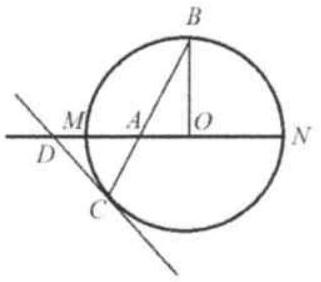
\includegraphics[width=\textwidth]{images/154(3).jpg}

\section*{Solution}
Connect \(O C\). Since \(O B=O C, \angle O B C=\angle O C B=\alpha\).\\
Since \(B O \perp M N\) and \(C D \perp O C, \angle D C O=\angle A O B=90^{\circ}\),

We see that \(\angle O A B=\angle D A C=90^{\circ}-\alpha=\beta\) and \(\angle D C A=90^{\circ}-\alpha=\beta\).

Thus \(\angle D C A=\angle D A C=\beta\), and \(D C=D A\).\\
\centering
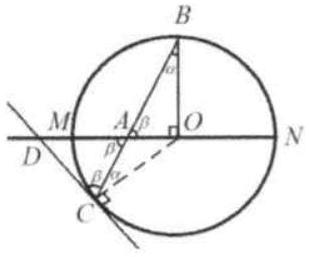
\includegraphics[width=\textwidth]{images/157(1).jpg}

\end{document}
